\documentclass[a4paper]{book}
\usepackage{makeidx}
\usepackage{graphicx}
\usepackage{multicol}
\usepackage{float}
\usepackage{listings}
\usepackage{color}
\usepackage{ifthen}
\usepackage[table]{xcolor}
\usepackage{textcomp}
\usepackage{alltt}
\usepackage{ifpdf}
\ifpdf
\usepackage[pdftex,
            pagebackref=true,
            colorlinks=true,
            linkcolor=blue,
            unicode
           ]{hyperref}
\else
\usepackage[ps2pdf,
            pagebackref=true,
            colorlinks=true,
            linkcolor=blue,
            unicode
           ]{hyperref}
\usepackage{pspicture}
\fi
\usepackage[utf8]{inputenc}
\usepackage{mathptmx}
\usepackage[scaled=.90]{helvet}
\usepackage{courier}
\usepackage{doxygen}
\lstset{language=C++,inputencoding=utf8,basicstyle=\footnotesize,breaklines=true,breakatwhitespace=true,tabsize=8,numbers=left }
\makeindex
\setcounter{tocdepth}{3}
\renewcommand{\footrulewidth}{0.4pt}
\begin{document}
\hypersetup{pageanchor=false}
\begin{titlepage}
\vspace*{7cm}
\begin{center}
{\Large Reference Manual}\\
\vspace*{1cm}
{\large Generated by Doxygen 1.7.3}\\
\vspace*{0.5cm}
{\small Wed Sep 19 2012 15:51:28}\\
\end{center}
\end{titlepage}
\clearemptydoublepage
\pagenumbering{roman}
\tableofcontents
\clearemptydoublepage
\pagenumbering{arabic}
\hypersetup{pageanchor=true}
\chapter{Class Index}
\section{Class Hierarchy}
This inheritance list is sorted roughly, but not completely, alphabetically:\begin{DoxyCompactList}
\item \contentsline{section}{Hylas::BaseType}{\pageref{structHylas_1_1BaseType}}{}
\begin{DoxyCompactList}
\item \contentsline{section}{Hylas::Type}{\pageref{structHylas_1_1Type}}{}
\begin{DoxyCompactList}
\item \contentsline{section}{Hylas::Generic}{\pageref{structHylas_1_1Generic}}{}
\end{DoxyCompactList}
\end{DoxyCompactList}
\item \contentsline{section}{BaseType}{\pageref{structBaseType}}{}
\begin{DoxyCompactList}
\item \contentsline{section}{Type}{\pageref{structType}}{}
\begin{DoxyCompactList}
\item \contentsline{section}{Generic}{\pageref{structGeneric}}{}
\end{DoxyCompactList}
\end{DoxyCompactList}
\item \contentsline{section}{Hylas::Compiler}{\pageref{structHylas_1_1Compiler}}{}
\item \contentsline{section}{Hylas::Form}{\pageref{structHylas_1_1Form}}{}
\item \contentsline{section}{Hylas::Lambda}{\pageref{structHylas_1_1Lambda}}{}
\item \contentsline{section}{Lambda}{\pageref{structLambda}}{}
\item \contentsline{section}{MetaFunction}{\pageref{structMetaFunction}}{}
\item \contentsline{section}{Hylas::MetaFunction}{\pageref{structHylas_1_1MetaFunction}}{}
\item \contentsline{section}{Hylas::Variable}{\pageref{structHylas_1_1Variable}}{}
\end{DoxyCompactList}

\chapter{Class Index}
\section{Class List}
Here are the classes, structs, unions and interfaces with brief descriptions:\begin{DoxyCompactList}
\item\contentsline{section}{\hyperlink{structHylas_1_1BaseType}{Hylas::BaseType} }{\pageref{structHylas_1_1BaseType}}{}
\item\contentsline{section}{\hyperlink{structBaseType}{BaseType} }{\pageref{structBaseType}}{}
\item\contentsline{section}{\hyperlink{structHylas_1_1Compiler}{Hylas::Compiler} }{\pageref{structHylas_1_1Compiler}}{}
\item\contentsline{section}{\hyperlink{structHylas_1_1Form}{Hylas::Form} }{\pageref{structHylas_1_1Form}}{}
\item\contentsline{section}{\hyperlink{structHylas_1_1Generic}{Hylas::Generic} }{\pageref{structHylas_1_1Generic}}{}
\item\contentsline{section}{\hyperlink{structGeneric}{Generic} }{\pageref{structGeneric}}{}
\item\contentsline{section}{\hyperlink{structHylas_1_1Lambda}{Hylas::Lambda} }{\pageref{structHylas_1_1Lambda}}{}
\item\contentsline{section}{\hyperlink{structLambda}{Lambda} }{\pageref{structLambda}}{}
\item\contentsline{section}{\hyperlink{structMetaFunction}{MetaFunction} }{\pageref{structMetaFunction}}{}
\item\contentsline{section}{\hyperlink{structHylas_1_1MetaFunction}{Hylas::MetaFunction} }{\pageref{structHylas_1_1MetaFunction}}{}
\item\contentsline{section}{\hyperlink{structHylas_1_1Type}{Hylas::Type} }{\pageref{structHylas_1_1Type}}{}
\item\contentsline{section}{\hyperlink{structType}{Type} }{\pageref{structType}}{}
\item\contentsline{section}{\hyperlink{structHylas_1_1Variable}{Hylas::Variable} }{\pageref{structHylas_1_1Variable}}{}
\end{DoxyCompactList}

\chapter{Class Documentation}
\hypertarget{structHylas_1_1BaseType}{
\section{Hylas::BaseType Struct Reference}
\label{structHylas_1_1BaseType}\index{Hylas::BaseType@{Hylas::BaseType}}
}
Inheritance diagram for Hylas::BaseType:\begin{figure}[H]
\begin{center}
\leavevmode
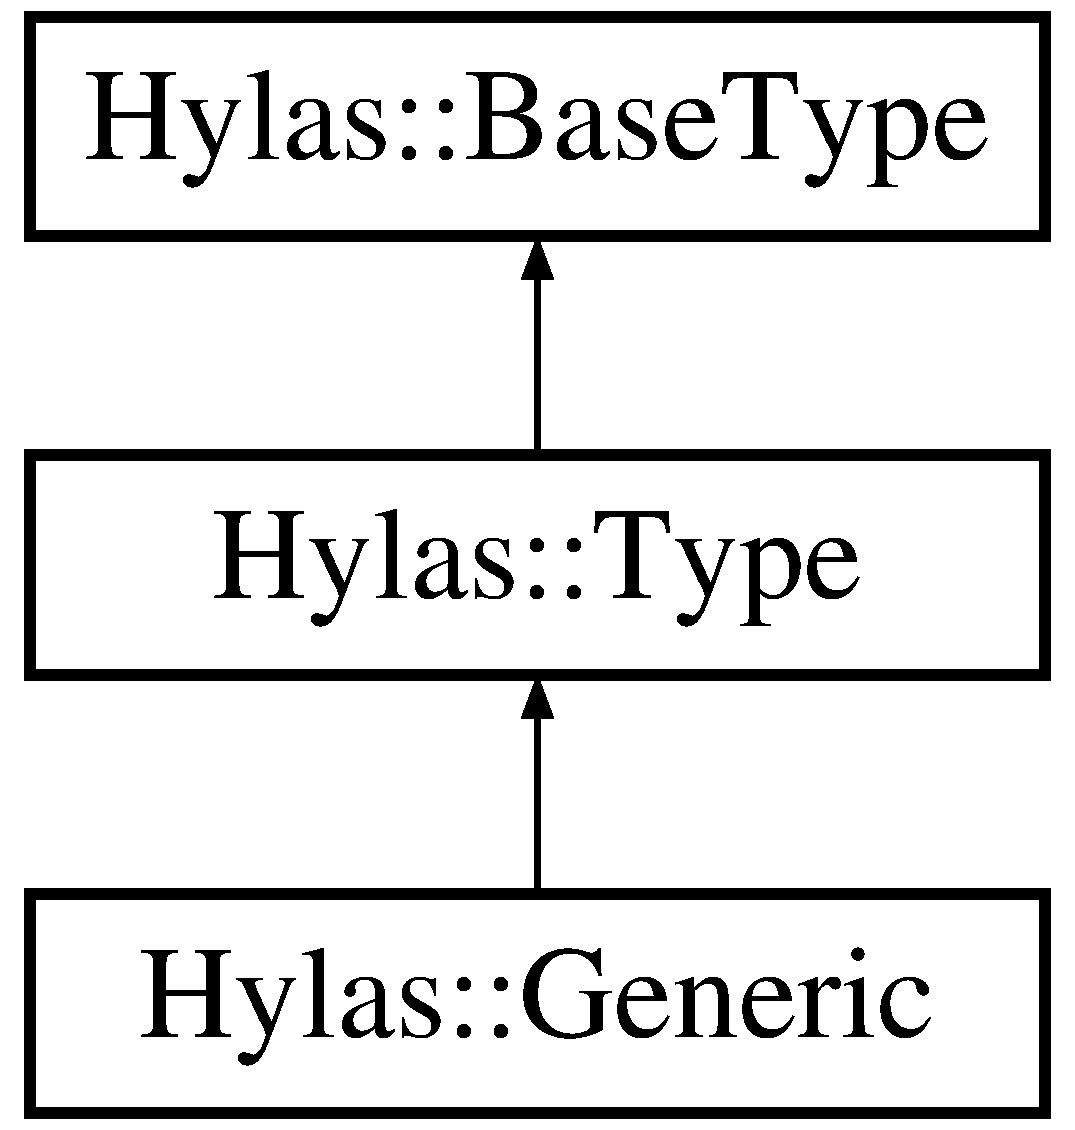
\includegraphics[height=3.000000cm]{structHylas_1_1BaseType}
\end{center}
\end{figure}
\subsection*{Public Attributes}
\begin{DoxyCompactItemize}
\item 
\hypertarget{structHylas_1_1BaseType_a77356f3ed9464a96a5b0a1a01376c9d2}{
unsigned char {\bfseries id}}
\label{structHylas_1_1BaseType_a77356f3ed9464a96a5b0a1a01376c9d2}

\end{DoxyCompactItemize}


The documentation for this struct was generated from the following file:\begin{DoxyCompactItemize}
\item 
types.hpp\end{DoxyCompactItemize}

\hypertarget{structBaseType}{
\section{BaseType Struct Reference}
\label{structBaseType}\index{BaseType@{BaseType}}
}
Inheritance diagram for BaseType:\begin{figure}[H]
\begin{center}
\leavevmode
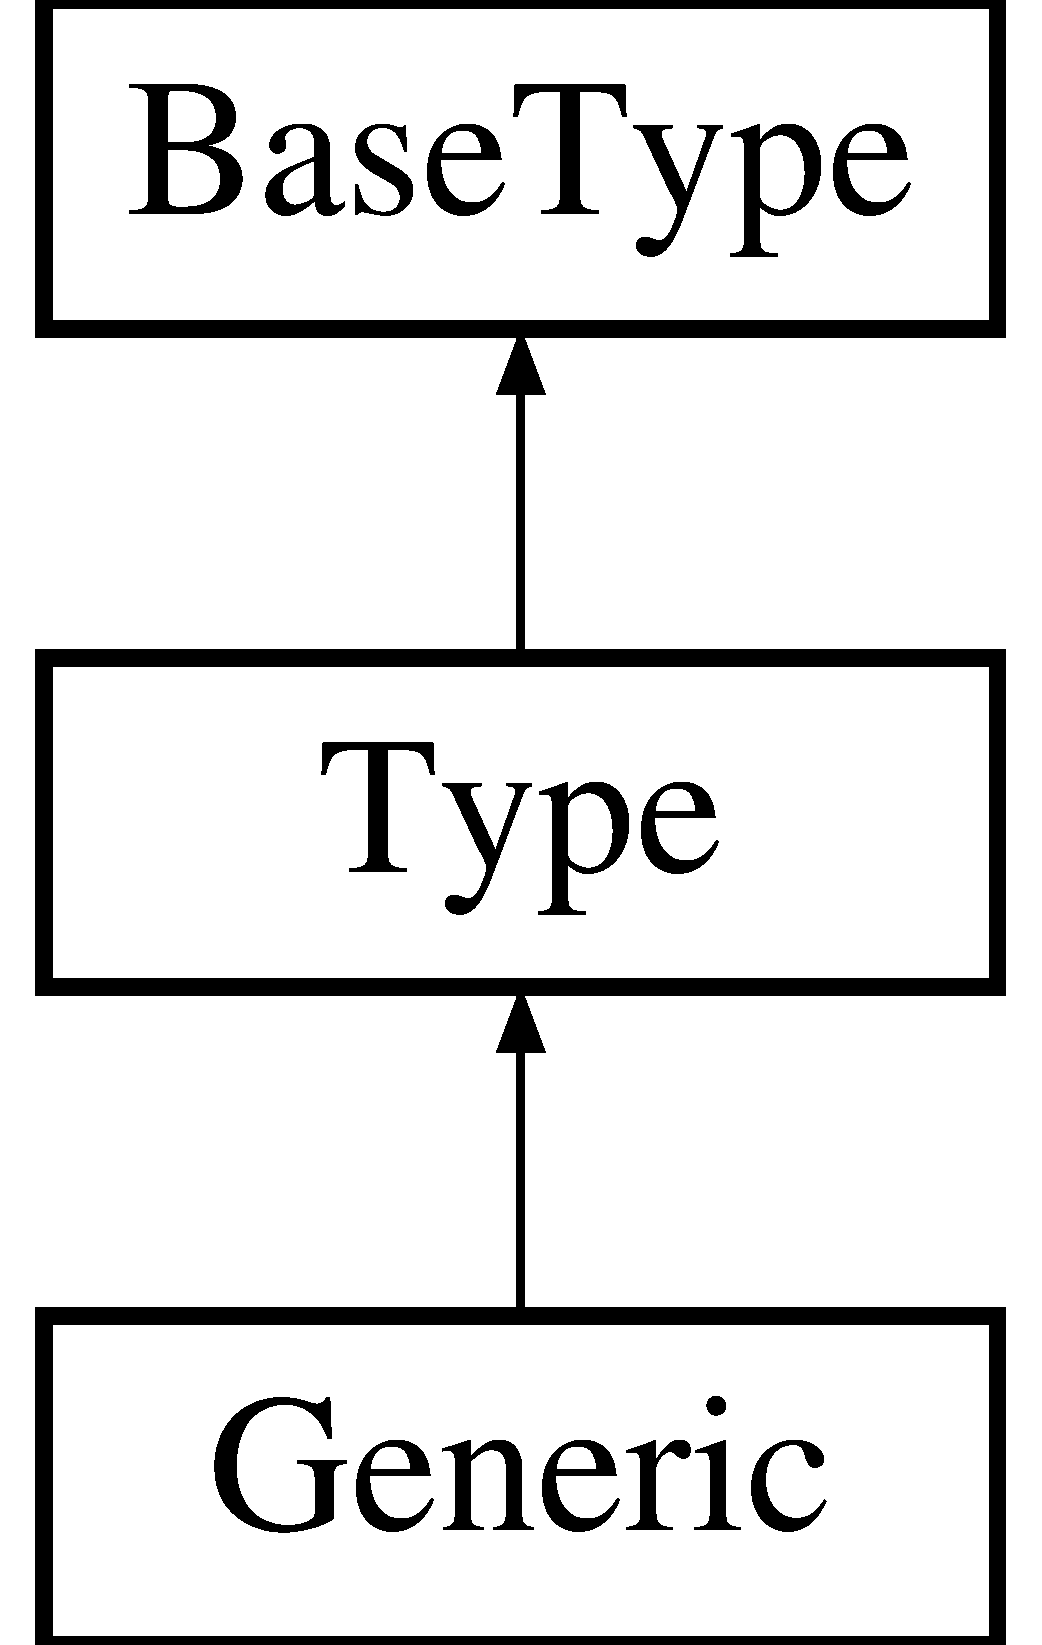
\includegraphics[height=3.000000cm]{structBaseType}
\end{center}
\end{figure}
\subsection*{Public Attributes}
\begin{DoxyCompactItemize}
\item 
\hypertarget{structBaseType_a520f7102b6261113b5f601b2247b7f55}{
unsigned char {\bfseries id}}
\label{structBaseType_a520f7102b6261113b5f601b2247b7f55}

\end{DoxyCompactItemize}


The documentation for this struct was generated from the following file:\begin{DoxyCompactItemize}
\item 
types.hpp\end{DoxyCompactItemize}

\hypertarget{structHylas_1_1Compiler}{
\section{Hylas::Compiler Struct Reference}
\label{structHylas_1_1Compiler}\index{Hylas::Compiler@{Hylas::Compiler}}
}
\subsection*{Public Attributes}
\begin{DoxyCompactItemize}
\item 
\hypertarget{structHylas_1_1Compiler_aef8902bd1771b058ccf8b89dc4d9f259}{
bool {\bfseries allow\_\-RedefineMacros}}
\label{structHylas_1_1Compiler_aef8902bd1771b058ccf8b89dc4d9f259}

\item 
\hypertarget{structHylas_1_1Compiler_ae256c9e84324dd6f6b595400aeefa7ad}{
bool {\bfseries allow\_\-RedefineFunctions}}
\label{structHylas_1_1Compiler_ae256c9e84324dd6f6b595400aeefa7ad}

\item 
\hypertarget{structHylas_1_1Compiler_ac5a42b0126cdcf422c70db422d4c2bc9}{
bool {\bfseries output}}
\label{structHylas_1_1Compiler_ac5a42b0126cdcf422c70db422d4c2bc9}

\end{DoxyCompactItemize}


The documentation for this struct was generated from the following file:\begin{DoxyCompactItemize}
\item 
hylas.hpp\end{DoxyCompactItemize}

\hypertarget{structHylas_1_1Form}{
\section{Hylas::Form Struct Reference}
\label{structHylas_1_1Form}\index{Hylas::Form@{Hylas::Form}}
}
\subsection*{Public Attributes}
\begin{DoxyCompactItemize}
\item 
\hypertarget{structHylas_1_1Form_a7504b9866df3e3c436cc67441648aeb4}{
bool {\bfseries Tag}}
\label{structHylas_1_1Form_a7504b9866df3e3c436cc67441648aeb4}

\item 
\hypertarget{structHylas_1_1Form_ad98691a6d2b3b38801bb1ff43ce911e3}{
string {\bfseries Value}}
\label{structHylas_1_1Form_ad98691a6d2b3b38801bb1ff43ce911e3}

\item 
\hypertarget{structHylas_1_1Form_ad9fae7fd1e22557687ab2a0824a6bdf0}{
\hyperlink{structHylas_1_1Form}{Form} $\ast$ {\bfseries Car}}
\label{structHylas_1_1Form_ad9fae7fd1e22557687ab2a0824a6bdf0}

\item 
\hypertarget{structHylas_1_1Form_a0750ded0ffad03b041d0c1aac5dfb710}{
\hyperlink{structHylas_1_1Form}{Form} $\ast$ {\bfseries Cdr}}
\label{structHylas_1_1Form_a0750ded0ffad03b041d0c1aac5dfb710}

\item 
\hypertarget{structHylas_1_1Form_a427709d4997a3162de8ee4aaba56708f}{
long {\bfseries line}}
\label{structHylas_1_1Form_a427709d4997a3162de8ee4aaba56708f}

\item 
\hypertarget{structHylas_1_1Form_afc8b8f6081e5d5287caabf254c524e14}{
int {\bfseries column}}
\label{structHylas_1_1Form_afc8b8f6081e5d5287caabf254c524e14}

\end{DoxyCompactItemize}


The documentation for this struct was generated from the following file:\begin{DoxyCompactItemize}
\item 
hylas.hpp\end{DoxyCompactItemize}

\hypertarget{structHylas_1_1Generic}{
\section{Hylas::Generic Struct Reference}
\label{structHylas_1_1Generic}\index{Hylas::Generic@{Hylas::Generic}}
}
Inheritance diagram for Hylas::Generic:\begin{figure}[H]
\begin{center}
\leavevmode
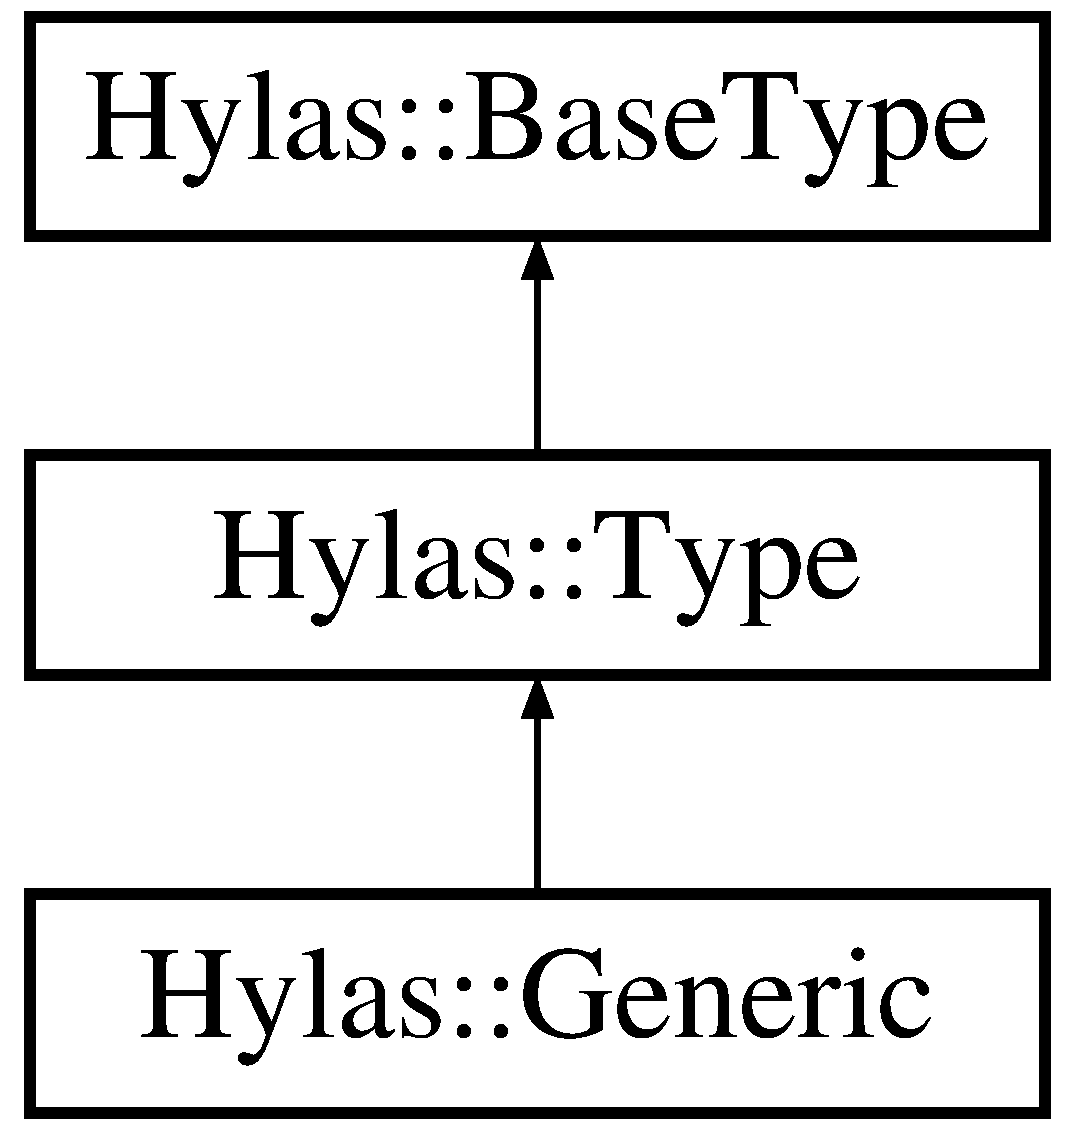
\includegraphics[height=3.000000cm]{structHylas_1_1Generic}
\end{center}
\end{figure}
\subsection*{Public Attributes}
\begin{DoxyCompactItemize}
\item 
\hypertarget{structHylas_1_1Generic_a9bd83e850da209025f98774a70b852aa}{
vector$<$ string $>$ {\bfseries arguments}}
\label{structHylas_1_1Generic_a9bd83e850da209025f98774a70b852aa}

\item 
\hypertarget{structHylas_1_1Generic_a5484587d04ff1b1d45f1efa755d904ce}{
\hyperlink{structHylas_1_1Form}{Form} $\ast$ {\bfseries code}}
\label{structHylas_1_1Generic_a5484587d04ff1b1d45f1efa755d904ce}

\item 
\hypertarget{structHylas_1_1Generic_a27d274c995fd29906050544309b083c2}{
map$<$ string, map$<$ string, pair$<$ long, string $>$ $>$ $>$ {\bfseries specializations}}
\label{structHylas_1_1Generic_a27d274c995fd29906050544309b083c2}

\item 
\hypertarget{structHylas_1_1Generic_ae8ceb9857d624ca16df1529763b69fd4}{
vector$<$ \hyperlink{structHylas_1_1Form}{Form} $\ast$ $>$ {\bfseries methods}}
\label{structHylas_1_1Generic_ae8ceb9857d624ca16df1529763b69fd4}

\end{DoxyCompactItemize}


The documentation for this struct was generated from the following file:\begin{DoxyCompactItemize}
\item 
types.hpp\end{DoxyCompactItemize}

\hypertarget{structGeneric}{
\section{Generic Struct Reference}
\label{structGeneric}\index{Generic@{Generic}}
}
Inheritance diagram for Generic:\begin{figure}[H]
\begin{center}
\leavevmode
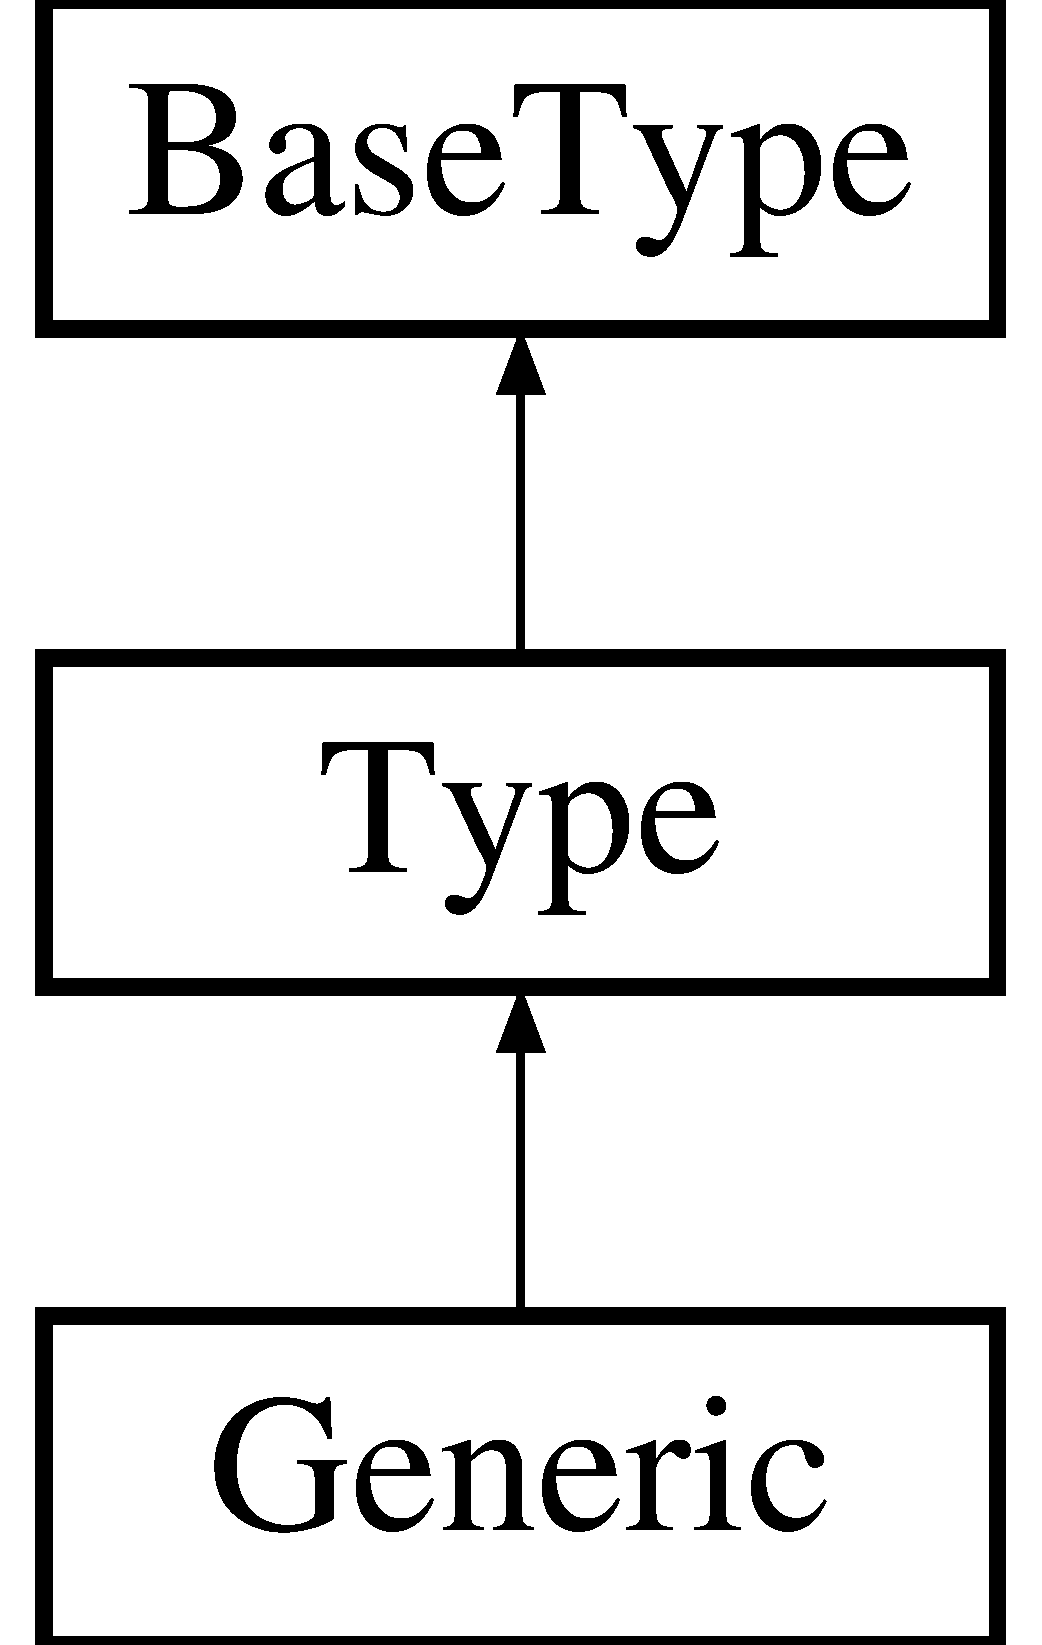
\includegraphics[height=3.000000cm]{structGeneric}
\end{center}
\end{figure}
\subsection*{Public Attributes}
\begin{DoxyCompactItemize}
\item 
\hypertarget{structGeneric_ad048043d5daa89f7d36f573b3ce515c1}{
vector$<$ string $>$ {\bfseries arguments}}
\label{structGeneric_ad048043d5daa89f7d36f573b3ce515c1}

\item 
\hypertarget{structGeneric_ab948d4a70418e0bc01d434a0be599486}{
Form $\ast$ {\bfseries code}}
\label{structGeneric_ab948d4a70418e0bc01d434a0be599486}

\item 
\hypertarget{structGeneric_a4518a5cdeed8d7ed927b2ac590e0e27a}{
map$<$ string, map$<$ string, pair$<$ long, string $>$ $>$ $>$ {\bfseries specializations}}
\label{structGeneric_a4518a5cdeed8d7ed927b2ac590e0e27a}

\item 
\hypertarget{structGeneric_a610e8f55b60d655b85d9d027c74657dc}{
vector$<$ Form $\ast$ $>$ {\bfseries methods}}
\label{structGeneric_a610e8f55b60d655b85d9d027c74657dc}

\end{DoxyCompactItemize}


The documentation for this struct was generated from the following file:\begin{DoxyCompactItemize}
\item 
types.hpp\end{DoxyCompactItemize}

\hypertarget{structHylas_1_1Lambda}{
\section{Hylas::Lambda Struct Reference}
\label{structHylas_1_1Lambda}\index{Hylas::Lambda@{Hylas::Lambda}}
}
\subsection*{Public Attributes}
\begin{DoxyCompactItemize}
\item 
\hypertarget{structHylas_1_1Lambda_a12efa497114066848dd624bf52fda37d}{
string {\bfseries name}}
\label{structHylas_1_1Lambda_a12efa497114066848dd624bf52fda37d}

\item 
\hypertarget{structHylas_1_1Lambda_a1172a9a8b0f961d5f541182b1209792b}{
string {\bfseries ret\_\-type}}
\label{structHylas_1_1Lambda_a1172a9a8b0f961d5f541182b1209792b}

\item 
\hypertarget{structHylas_1_1Lambda_afc442e5b73f0603e3daf0535e41cf696}{
unsigned long {\bfseries nargs}}
\label{structHylas_1_1Lambda_afc442e5b73f0603e3daf0535e41cf696}

\item 
\hypertarget{structHylas_1_1Lambda_a124b3dfe66094876aa7682bb0dc8ec5e}{
map$<$ string, string $>$ {\bfseries arguments}}
\label{structHylas_1_1Lambda_a124b3dfe66094876aa7682bb0dc8ec5e}

\item 
\hypertarget{structHylas_1_1Lambda_a8b881211c7042316ced0dae3ef7f2a5f}{
bool {\bfseries fastcc}}
\label{structHylas_1_1Lambda_a8b881211c7042316ced0dae3ef7f2a5f}

\item 
\hypertarget{structHylas_1_1Lambda_af8975a872b39bde4d75c42d83e6ee6cb}{
bool {\bfseries tco}}
\label{structHylas_1_1Lambda_af8975a872b39bde4d75c42d83e6ee6cb}

\item 
\hypertarget{structHylas_1_1Lambda_ad30b10319eb86291d66026aaf0cb492b}{
bool {\bfseries lining}}
\label{structHylas_1_1Lambda_ad30b10319eb86291d66026aaf0cb492b}

\item 
\hypertarget{structHylas_1_1Lambda_a0c597e219180835bcf080d2a65b7f0df}{
string {\bfseries docstring}}
\label{structHylas_1_1Lambda_a0c597e219180835bcf080d2a65b7f0df}

\end{DoxyCompactItemize}


The documentation for this struct was generated from the following file:\begin{DoxyCompactItemize}
\item 
fndef.hpp\end{DoxyCompactItemize}

\hypertarget{structLambda}{
\section{Lambda Struct Reference}
\label{structLambda}\index{Lambda@{Lambda}}
}
\subsection*{Public Attributes}
\begin{DoxyCompactItemize}
\item 
\hypertarget{structLambda_a289f62f08113ee05dcd6038f5785549e}{
string {\bfseries name}}
\label{structLambda_a289f62f08113ee05dcd6038f5785549e}

\item 
\hypertarget{structLambda_a2e0271d03ceaa0cf02b92f570ed86637}{
string {\bfseries ret\_\-type}}
\label{structLambda_a2e0271d03ceaa0cf02b92f570ed86637}

\item 
\hypertarget{structLambda_ace6dd93e8972c2abf820f6875c1cb53b}{
unsigned long {\bfseries nargs}}
\label{structLambda_ace6dd93e8972c2abf820f6875c1cb53b}

\item 
\hypertarget{structLambda_a3e41ab2e01aa054ea49e01bddb14f7af}{
map$<$ string, string $>$ {\bfseries arguments}}
\label{structLambda_a3e41ab2e01aa054ea49e01bddb14f7af}

\item 
\hypertarget{structLambda_a768b3c61cc18d43b9e4d54312611b653}{
bool {\bfseries fastcc}}
\label{structLambda_a768b3c61cc18d43b9e4d54312611b653}

\item 
\hypertarget{structLambda_a0023c87f80cd4b7cac05d8b0517fd0ee}{
bool {\bfseries tco}}
\label{structLambda_a0023c87f80cd4b7cac05d8b0517fd0ee}

\item 
\hypertarget{structLambda_ac3e3d2559f4b95571d6e6a6fc4fddea8}{
bool {\bfseries lining}}
\label{structLambda_ac3e3d2559f4b95571d6e6a6fc4fddea8}

\item 
\hypertarget{structLambda_aadf382267d79bc1c5146bf666f9d216e}{
string {\bfseries docstring}}
\label{structLambda_aadf382267d79bc1c5146bf666f9d216e}

\end{DoxyCompactItemize}


The documentation for this struct was generated from the following file:\begin{DoxyCompactItemize}
\item 
fndef.hpp\end{DoxyCompactItemize}

\hypertarget{structMetaFunction}{
\section{MetaFunction Struct Reference}
\label{structMetaFunction}\index{MetaFunction@{MetaFunction}}
}
\subsection*{Public Attributes}
\begin{DoxyCompactItemize}
\item 
\hypertarget{structMetaFunction_a66e5f923e15ce7d66b371a2387f8c94c}{
vector$<$ \hyperlink{structLambda}{Lambda} $>$ {\bfseries versions}}
\label{structMetaFunction_a66e5f923e15ce7d66b371a2387f8c94c}

\end{DoxyCompactItemize}


The documentation for this struct was generated from the following file:\begin{DoxyCompactItemize}
\item 
fndef.hpp\end{DoxyCompactItemize}

\hypertarget{structHylas_1_1MetaFunction}{
\section{Hylas::MetaFunction Struct Reference}
\label{structHylas_1_1MetaFunction}\index{Hylas::MetaFunction@{Hylas::MetaFunction}}
}
\subsection*{Public Attributes}
\begin{DoxyCompactItemize}
\item 
\hypertarget{structHylas_1_1MetaFunction_ac7edbc968d651f86d5b140ccbd47f18d}{
vector$<$ \hyperlink{structHylas_1_1Lambda}{Lambda} $>$ {\bfseries versions}}
\label{structHylas_1_1MetaFunction_ac7edbc968d651f86d5b140ccbd47f18d}

\end{DoxyCompactItemize}


The documentation for this struct was generated from the following file:\begin{DoxyCompactItemize}
\item 
fndef.hpp\end{DoxyCompactItemize}

\hypertarget{structHylas_1_1Type}{
\section{Hylas::Type Struct Reference}
\label{structHylas_1_1Type}\index{Hylas::Type@{Hylas::Type}}
}
Inheritance diagram for Hylas::Type:\begin{figure}[H]
\begin{center}
\leavevmode
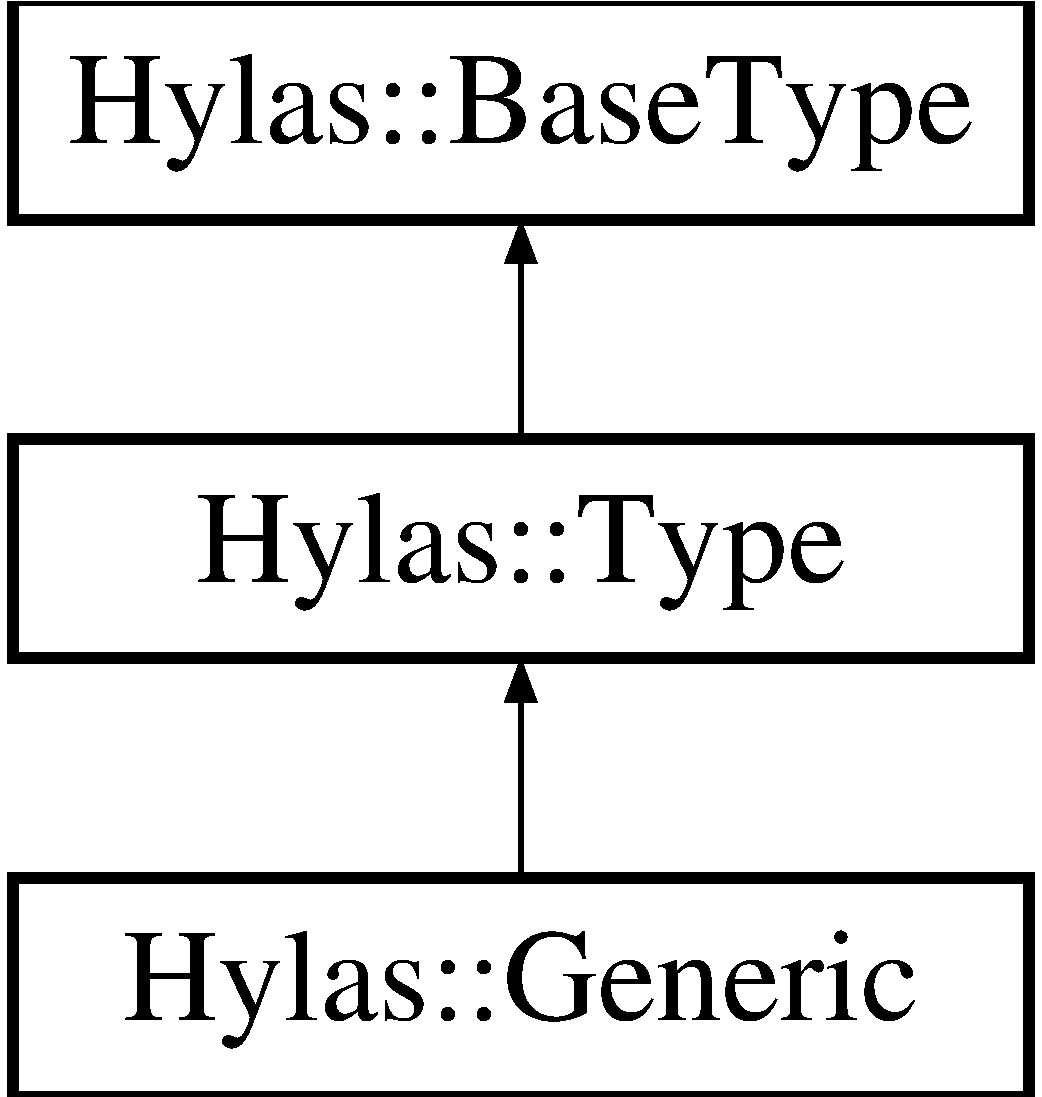
\includegraphics[height=3.000000cm]{structHylas_1_1Type}
\end{center}
\end{figure}
\subsection*{Public Attributes}
\begin{DoxyCompactItemize}
\item 
\hypertarget{structHylas_1_1Type_a28ed2feb5ad8a07dd272c8408c7cbb7f}{
map$<$ string, pair$<$ long, string $>$ $>$ {\bfseries members}}
\label{structHylas_1_1Type_a28ed2feb5ad8a07dd272c8408c7cbb7f}

\end{DoxyCompactItemize}


The documentation for this struct was generated from the following file:\begin{DoxyCompactItemize}
\item 
types.hpp\end{DoxyCompactItemize}

\hypertarget{structType}{
\section{Type Struct Reference}
\label{structType}\index{Type@{Type}}
}
Inheritance diagram for Type:\begin{figure}[H]
\begin{center}
\leavevmode
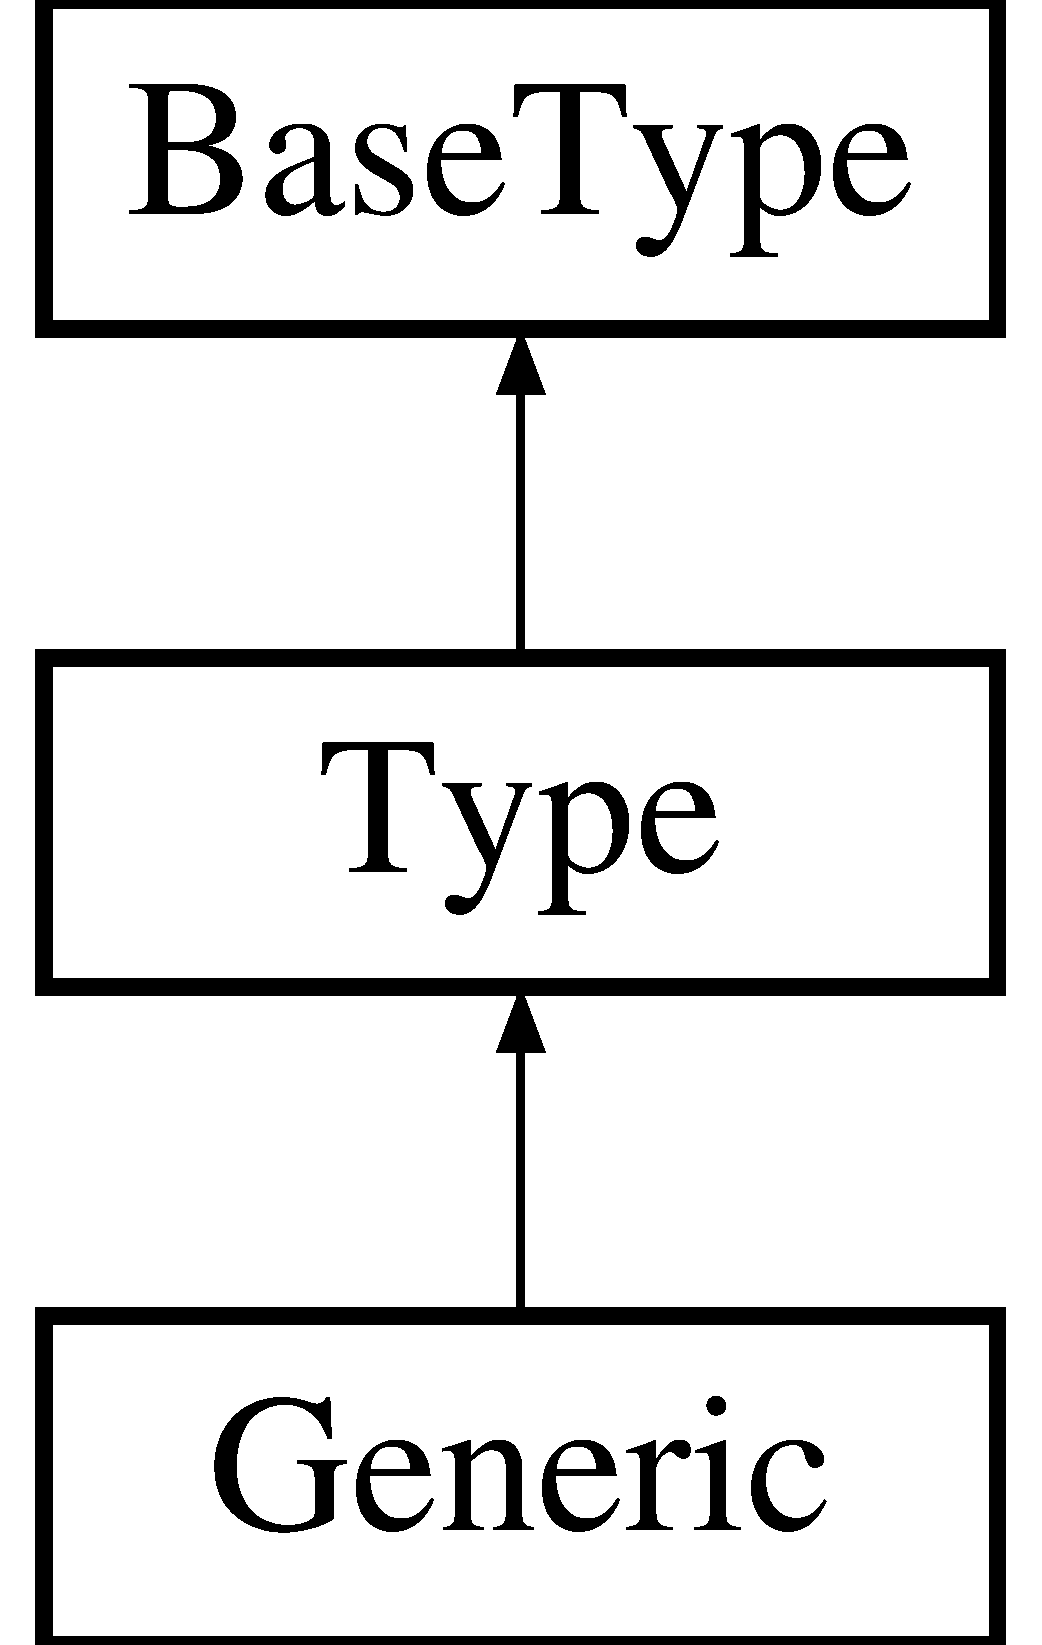
\includegraphics[height=3.000000cm]{structType}
\end{center}
\end{figure}
\subsection*{Public Attributes}
\begin{DoxyCompactItemize}
\item 
\hypertarget{structType_a3e5a92ad7e9ed15e37cbf400a835eea5}{
map$<$ string, pair$<$ long, string $>$ $>$ {\bfseries members}}
\label{structType_a3e5a92ad7e9ed15e37cbf400a835eea5}

\end{DoxyCompactItemize}


The documentation for this struct was generated from the following file:\begin{DoxyCompactItemize}
\item 
types.hpp\end{DoxyCompactItemize}

\hypertarget{structHylas_1_1Variable}{
\section{Hylas::Variable Struct Reference}
\label{structHylas_1_1Variable}\index{Hylas::Variable@{Hylas::Variable}}
}
\subsection*{Public Attributes}
\begin{DoxyCompactItemize}
\item 
\hypertarget{structHylas_1_1Variable_afb6c3449837e7b9de6b174de9ab08436}{
media sda3 Code Hylas src hylas hpp string {\bfseries sym}}
\label{structHylas_1_1Variable_afb6c3449837e7b9de6b174de9ab08436}

\item 
\hypertarget{structHylas_1_1Variable_a6d303ea037f5535b572e0eadf55ddba2}{
bool {\bfseries constant}}
\label{structHylas_1_1Variable_a6d303ea037f5535b572e0eadf55ddba2}

\item 
\hypertarget{structHylas_1_1Variable_aae7ee4de7e5504443ca99fd7b0ff676c}{
bool {\bfseries argument}}
\label{structHylas_1_1Variable_aae7ee4de7e5504443ca99fd7b0ff676c}

\end{DoxyCompactItemize}


The documentation for this struct was generated from the following file:\begin{DoxyCompactItemize}
\item 
hylas.hpp\end{DoxyCompactItemize}

\printindex
\end{document}
